% Provenance (never printed): cycle 4 SVT, "La planete Terre, l'environnement
% et l'action humaine": climate, its past variations and the present change,
% read from data; see sources/book1/PROVENANCE.md. Book 1, grade 9, chapter 1.
% Vocabulary guard: owns climate change (first look; Book 2 g12 re-uses it),
% global warming, temperature anomaly. The greenhouse effect and greenhouse
% gases belong to the chemistry series (grade 8): recalled in prose, never
% defined. Infrared is physics (g10): named in prose only. "Glacial period"
% and "interglacial" belong to Book 2 g12: here "the ice ages and the warmer
% times between them". Physical science only, in the IPCC's calibrated words;
% no policy.
\chapter{पृथ्वी की जलवायु, अतीत और वर्तमान}\label{ch:g9:climate-past-and-present}

अगर पृथ्वी के चारों ओर कोई हवा न होती, पर वह सूर्य के प्रकाश का उतना ही हिस्सा परावर्तित
करती जितना आज करती है, तो उसकी सतह लगभग \qty{-19}{\degreeCelsius} के औसत तापमान पर
टिक जाती: हर जगह जमे \omterm{def:g2:water-on-earth:ocean}{समुद्र}, जमी ज़मीन। उसका असली औसत लगभग \qty{15}{\degreeCelsius}
है। यह अंतर, कोई \qty{34}{\degreeCelsius}, हवा में बहुत कम मात्रा में मौजूद कुछ गैसों
से आता है, जो पृथ्वी की ऊष्मा के एक हिस्से को अंतरिक्ष में निकलने से रोकती हैं। यह
अध्याय इन गैसों के बारे में है, अतीत में पृथ्वी की \omterm{def:g5:weather-and-climate:climate}{जलवायु} के बारे में है, और इस बारे में
है कि वह अब कैसे और क्यों बदल रही है।
% ledger: earth:Tbb, earth:Tsurf (figdata/grade-9/climate_records.py: -19.1 and 14.9 degC, gap 34)

\begin{recall}
किसी जगह की \omterm{def:g5:weather-and-climate:climate}{जलवायु} वह \omterm{def:g1:watching-the-weather:weather}{मौसम} है जो वहाँ आमतौर पर होता है, 30 वर्षों का औसत लेकर
(\cref{ch:g5:weather-and-climate})। वायुमंडल की सबसे निचली परत, जहाँ \omterm{def:g1:watching-the-weather:weather}{मौसम} होता है,
\omterm{def:g8:the-atmosphere:layers}{क्षोभमंडल} है (\cref{ch:g8:the-atmosphere})। \omterm{def:g8:ice-on-earth:ice-age}{हिमयुग}, \omterm{def:g3:continents-and-oceans:poles}{ध्रुवों} से बहुत आगे तक फैली
\omterm{def:g8:ice-on-earth:ice-sheet}{हिमचादरों} के साथ, आते-जाते रहे हैं; आर्कटिक की \omterm{def:g8:ice-on-earth:sea-ice}{समुद्री बर्फ़} 1979 से सिकुड़ी है
(\cref{ch:g8:ice-on-earth})। रसायन विज्ञान में तुम सीखते हो कि कार्बन डाइऑक्साइड,
मीथेन और जलवाष्प \emph{ग्रीनहाउस गैसें} हैं: वे सूर्य के प्रकाश को गुज़रने देती हैं पर
गरम ज़मीन से निकलने वाले अदृश्य अवरक्त प्रकाश को सोख लेती हैं, जो \emph{ग्रीनहाउस
प्रभाव} है; कोयला, तेल और गैस जलाने से कार्बन डाइऑक्साइड निकलती
है।
\end{recall}

\section{ग्रीनहाउस प्रभाव और पृथ्वी का तापमान}

सूर्य का प्रकाश वायुमंडल पार करता है और ज़मीन और \omterm{def:g2:water-on-earth:ocean}{महासागरों} को गरम करता है। हर गरम
पिंड की तरह, गरम सतह बदले में ऊर्जा छोड़ती है, अवरक्त प्रकाश के रूप में, जिसे आँख नहीं
देख सकती। अगर यह सारी ऊर्जा अंतरिक्ष में निकल जाती, तो पृथ्वी पहले अनुच्छेद की जमी हुई
दुनिया होती। पर हवा की ग्रीनहाउस गैसें इस अवरक्त प्रकाश का बहुत-सा हिस्सा सोख लेती हैं
और उसका एक भाग वापस नीचे भेजती हैं: सतह को सूर्य से भी और अपने ऊपर की हवा से भी ऊर्जा
मिलती है, और वह एक ज़्यादा ऊँचे तापमान पर टिक जाती
है।

\begin{omfigure}
\begin{tikzpicture}[font=\footnotesize, >={Stealth[length=2.4mm]}]
  % ground and atmosphere
  \fill[omLithAlluv] (0,0) rectangle (12,0.5);
  \fill[omSea!45] (0,0.5) rectangle (12,3.4);
  \node[anchor=north east, align=right] at (11.85,3.35) {ग्रीनहाउस गैसों\\ वाला वायुमंडल};
  \node[anchor=south east] at (11.9,0.05) {ज़मीन और महासागर};
  \node[anchor=south west] at (0.15,3.5) {अंतरिक्ष};
  % Sun
  \fill[omWxSun] (1.3,5.0) circle (0.45);
  \node at (1.3,4.3) {सूर्य};
  % sunlight in
  \draw[->, omWxSun!80!black, line width=2.2pt] (1.7,4.6) -- (2.7,0.55)
    node[pos=0.25, right=2pt, align=left, black] {सूर्य का प्रकाश आता है\\ और सतह को गरम करता है};
  % infrared out and back
  \draw[->, omWarm, line width=1.6pt, decorate, decoration={snake, amplitude=1mm, segment length=4mm, post length=3mm}]
    (6.0,0.55) -- (6.6,2.6);
  \draw[->, omWarm, line width=1.6pt, decorate, decoration={snake, amplitude=1mm, segment length=4mm, post length=3mm}]
    (6.6,2.7) -- (7.4,5.0) node[right, align=left, black] {एक हिस्सा अंतरिक्ष\\ में निकल जाता है};
  \draw[->, omWarm, line width=1.6pt, decorate, decoration={snake, amplitude=1mm, segment length=4mm, post length=3mm}]
    (6.8,2.75) -- (8.6,0.55);
  \node[align=left, anchor=west] at (8.8,1.9) {एक हिस्सा गैसें\\ सोखती हैं और\\ वापस नीचे भेजती हैं};
  \node[align=right, anchor=east] at (5.9,1.3) {गरम सतह\\ अवरक्त छोड़ती है};
\end{tikzpicture}

{\small ग्रीनहाउस प्रभाव, सरल रूप में (एक रेखाचित्र)। इसके बिना पृथ्वी की सतह का औसत
लगभग \qty{-19}{\degreeCelsius} होता; इसके साथ, लगभग
\qty{15}{\degreeCelsius}।}
% ledger: earth:Tbb, earth:Tsurf
\label{fig:g9:climate-past-and-present:greenhouse}
\end{omfigure}

ग्रीनहाउस प्रभाव प्राकृतिक और ज़रूरी है: इसके बिना सतह पर कोई तरल पानी न होता। इस
अध्याय का प्रश्न दूसरा है: जब हवा में ग्रीनहाउस गैस की मात्रा बदलती है, तो पृथ्वी के
तापमान के साथ क्या होता
है?

\section{अतीत की जलवायु}

सुदूर अतीत की \omterm{def:g5:weather-and-climate:climate}{जलवायु} पढ़ने के लिए वैज्ञानिक \omterm{def:g8:ice-on-earth:ice-sheet}{हिमचादरों} में छेद करते हैं। हर वर्ष
अंटार्कटिका और ग्रीनलैंड पर \omterm{def:g4:clouds-rain-snow:precipitation}{हिम} गिरता है, और गर्मी का \omterm{def:g4:clouds-rain-snow:precipitation}{हिम} जाड़े के \omterm{def:g4:clouds-rain-snow:precipitation}{हिम} से थोड़ा अलग होता
है। दबकर और भिंचकर बर्फ़ बनने पर भी वार्षिक परतें बची रहती हैं, एक के ऊपर एक, किसी
किताब के पन्नों की तरह। बर्फ़ जितनी गहरी, उतनी पुरानी।
% ledger: eo:ice-core

\begin{omfigure}
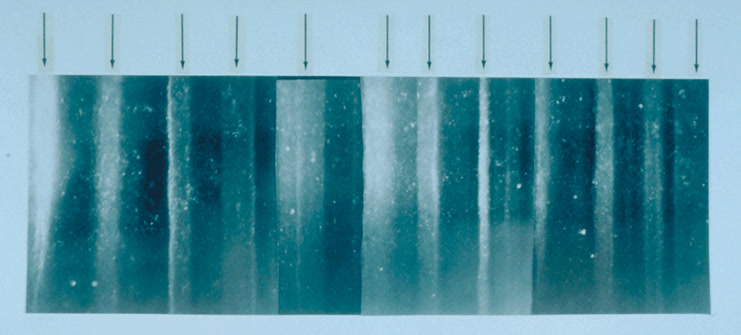
\includegraphics[width=0.78\linewidth]{images/book1/g9-gisp2-layers.jpg}

{\small बर्फ़ के एक कोर का \qty{19}{cm} लंबा हिस्सा, जिसे ग्रीनलैंड की \omterm{def:g8:ice-on-earth:ice-sheet}{हिमचादर} में
\qty{1855}{m} की गहराई पर छेदकर निकाला गया और नीचे से रोशनी डाली गई। तीर गहरी जाड़े की
परतों के बीच की हल्की गर्मी की परतों की ओर इशारा करते हैं: \omterm{def:g4:clouds-rain-snow:precipitation}{हिम} के ग्यारह वर्ष। NOAA
पुराजलवायु विज्ञान (सार्वजनिक डोमेन, विकिमीडिया
कॉमन्स के ज़रिए)।}
% ledger: commons:gisp2-layers
\label{fig:g9:climate-past-and-present:ice-core}
\end{omfigure}

बर्फ़ का कोर अतीत के दो अभिलेख रखता है। ख़ुद \omterm{def:g4:clouds-rain-snow:precipitation}{हिम} बताता है कि गिरते समय हवा कितनी ठंडी
थी: हवा जितनी ठंडी, \omterm{def:g4:clouds-rain-snow:precipitation}{हिम} में हाइड्रोजन और ऑक्सीजन के भारी रूपों का हिस्सा उतना कम। और
जब \omterm{def:g4:clouds-rain-snow:precipitation}{हिम} दबकर बर्फ़ बनता है, तो दानों के बीच की जगहें बंद हो जाती हैं, और उस समय की हवा
के नन्हे बुलबुले फँस जाते हैं। वैज्ञानिक प्रयोगशाला में इस प्राचीन हवा को निकालते हैं और
उसकी कार्बन डाइऑक्साइड मापते
हैं।
% ledger: eo:ice-core

\begin{omfigure}
\begin{tikzpicture}
\begin{axis}[name=temp, omrecord, omage, width=13cm, height=3.9cm, xmin=0, xmax=800,
  xtick={0,100,...,800}, xticklabels={}, ylabel={तापमान में\\ बदलाव ($^\circ$C)},
  ylabel style={align=center}, ymin=-11, ymax=5, ytick={-10,-5,0,5}]
  \addplot[omWarm, line width=0.7pt] table[x=age_kyr, y=temp_C] {figdata/out/grade-9-climate_records-edc.dat};
\end{axis}
\begin{axis}[at={(temp.south west)}, anchor=north west, yshift=-0.3cm, omrecord, omage,
  width=13cm, height=3.9cm, xmin=0, xmax=800, xtick={0,100,...,800},
  xlabel={आज से हज़ारों वर्ष पहले}, ylabel={कार्बन\\ डाइऑक्साइड (ppm)},
  ylabel style={align=center}, ymin=160, ymax=320, ytick={180,220,260,300}]
  \addplot[black, line width=0.7pt] table[x=age_kyr, y=co2_ppm] {figdata/out/grade-9-climate_records-icecore.dat};
\end{axis}
\end{tikzpicture}

{\small अंटार्कटिका की बर्फ़ में पढ़े गए आठ लाख वर्ष। ऊपर: डोम~C पर हवा के तापमान में
बदलाव, पिछले हज़ार वर्षों के औसत की तुलना में (EPICA डोम~C बर्फ़ कोर, ज़ूज़ेल और अन्य,
2007)। नीचे: बर्फ़ में फँसी हवा की कार्बन डाइऑक्साइड, प्रति दस लाख भाग में (बेराइटर और
अन्य, 2015)। दोनों का \num{2000} वर्षों के क़दमों पर औसत लिया गया है; समय बाईं ओर
(सबसे पुराना) से दाईं ओर (आज) चलता
है।}
% ledger: data:edc-jouzel, data:co2-bereiter (figdata/grade-9/climate_records.py)
\label{fig:g9:climate-past-and-present:icecore}
\end{omfigure}

दोनों वक्र एक ही कहानी कहते हैं। बार-बार लंबे ठंडे समय, यानी \omterm{def:g8:ice-on-earth:ice-age}{हिमयुग}, छोटे गरम समयों को
जगह देते रहे, फिर ठंड लौट आई। सबसे ठंडे समय में अंटार्कटिका के ऊपर की हवा पिछले हज़ार
वर्षों से लगभग \qty{9}{\degreeCelsius} ज़्यादा ठंडी थी; सबसे गरम समयों में वह कुछ डिग्री
ज़्यादा गरम थी। और कार्बन डाइऑक्साइड तापमान के साथ बढ़ती-घटती रही, ठंडे समयों में लगभग
\qty{175}{ppm} और गरम समयों में लगभग \qty{300}{ppm} के बीच। हम उन गरम समयों में से
एक में रहते हैं, जो पिछले \omterm{def:g8:ice-on-earth:ice-age}{हिमयुग} के ख़त्म होने पर शुरू
हुआ।
% ledger: data:edc-jouzel, data:co2-bereiter (figdata/grade-9/climate_records.py: edc min -9.7, max +3.6; CO2 174 to 299 ppm)

\begin{method}[दो अभिलेखों को साथ-साथ पढ़ना]
\begin{enumerate}
  \item जाँचो कि दोनों अभिलेखों का समय-अक्ष एक ही है, और समय किस ओर
        चलता है।
  \item समय-अक्ष पर एक तारीख़ चुनो और उस तारीख़ पर हर अभिलेख पढ़ो।
  \item शिखर और गर्त ढूँढो: क्या वे दोनों अभिलेखों में एक ही समय पर आते
        हैं?
  \item बताओ कि क्या साथ-साथ चलता है, अभी यह तय किए बिना कि किस बदलाव ने
        दूसरे को पैदा किया।
\end{enumerate}
\end{method}

\begin{example}[बर्फ़ के कोर में पिछला हिमयुग]
आज से \num{20000} वर्ष पहले (समय-अक्ष पर 20), तापमान का वक्र लगभग
\qty{-9}{\degreeCelsius} पर है और कार्बन डाइऑक्साइड लगभग \qty{190}{ppm} पर। पिछले
हज़ार वर्षों में तापमान का वक्र 0 के पास है और कार्बन डाइऑक्साइड \qty{280}{ppm} के
पास। तो, पिछले \omterm{def:g8:ice-on-earth:ice-age}{हिमयुग} के सबसे ठंडे समय में, अंटार्कटिका के ऊपर की हवा लगभग
\qty{9}{\degreeCelsius} ज़्यादा ठंडी थी, और उसमें लगभग
$280 - 190 = \qty{90}{ppm}$ कम कार्बन डाइऑक्साइड थी, एक तिहाई कम।
\end{example}
% ledger: data:edc-jouzel, data:co2-bereiter (figdata/grade-9/climate_records.py: 19-21 kyr bins -9.4, 190 ppm; 1 kyr bin 278)

और पीछे जाएँ तो पृथ्वी ने पिछले 800\,000 वर्षों के किसी भी समय से कहीं ज़्यादा गरम
\omterm{def:g5:weather-and-climate:climate}{जलवायु} देखी। वैज्ञानिक आकलनों का अनुमान है कि पिछली बार पृथ्वी की सतह उन्नीसवीं सदी के
अंत के अपने स्तर से \qty{2.5}{\degreeCelsius} या ज़्यादा ऊपर तीस लाख से भी ज़्यादा वर्ष
पहले रही थी।
% ledger: ipcc:3myr

\section{आज के अभिलेख}

उन्नीसवीं सदी के अंत से ज़मीन और \omterm{def:g2:water-on-earth:ocean}{समुद्र} पर हज़ारों \omterm{def:g4:clouds-rain-snow:weather-station}{मौसम केंद्रों} पर, छाया में रखे
थर्मामीटरों से, हर दिन तापमान मापा गया है। पूरे ग्रह को देखने के लिए वैज्ञानिक ख़ुद
तापमानों का औसत नहीं लेते, जो इस पर निर्भर करते हैं कि हर केंद्र कहाँ है, बल्कि इसका कि
हर एक अपने सामान्य मान से कितना अलग है।
% ledger: giss:method

\begin{definition}[तापमान विसंगति]\label{def:g9:climate-past-and-present:anomaly}
\emph{तापमान विसंगति}\index{तापमान विसंगति} किसी तापमान और एक चुनी हुई संदर्भ
अवधि में उसके औसत के बीच का अंतर है। जब \omterm{def:g1:watching-the-weather:weather}{मौसम} उस औसत से गरम हो तो वह धनात्मक होती है,
जब ठंडा हो तो
ऋणात्मक।
\end{definition}

\begin{omfigure}
\begin{minipage}[c]{0.44\linewidth}\centering
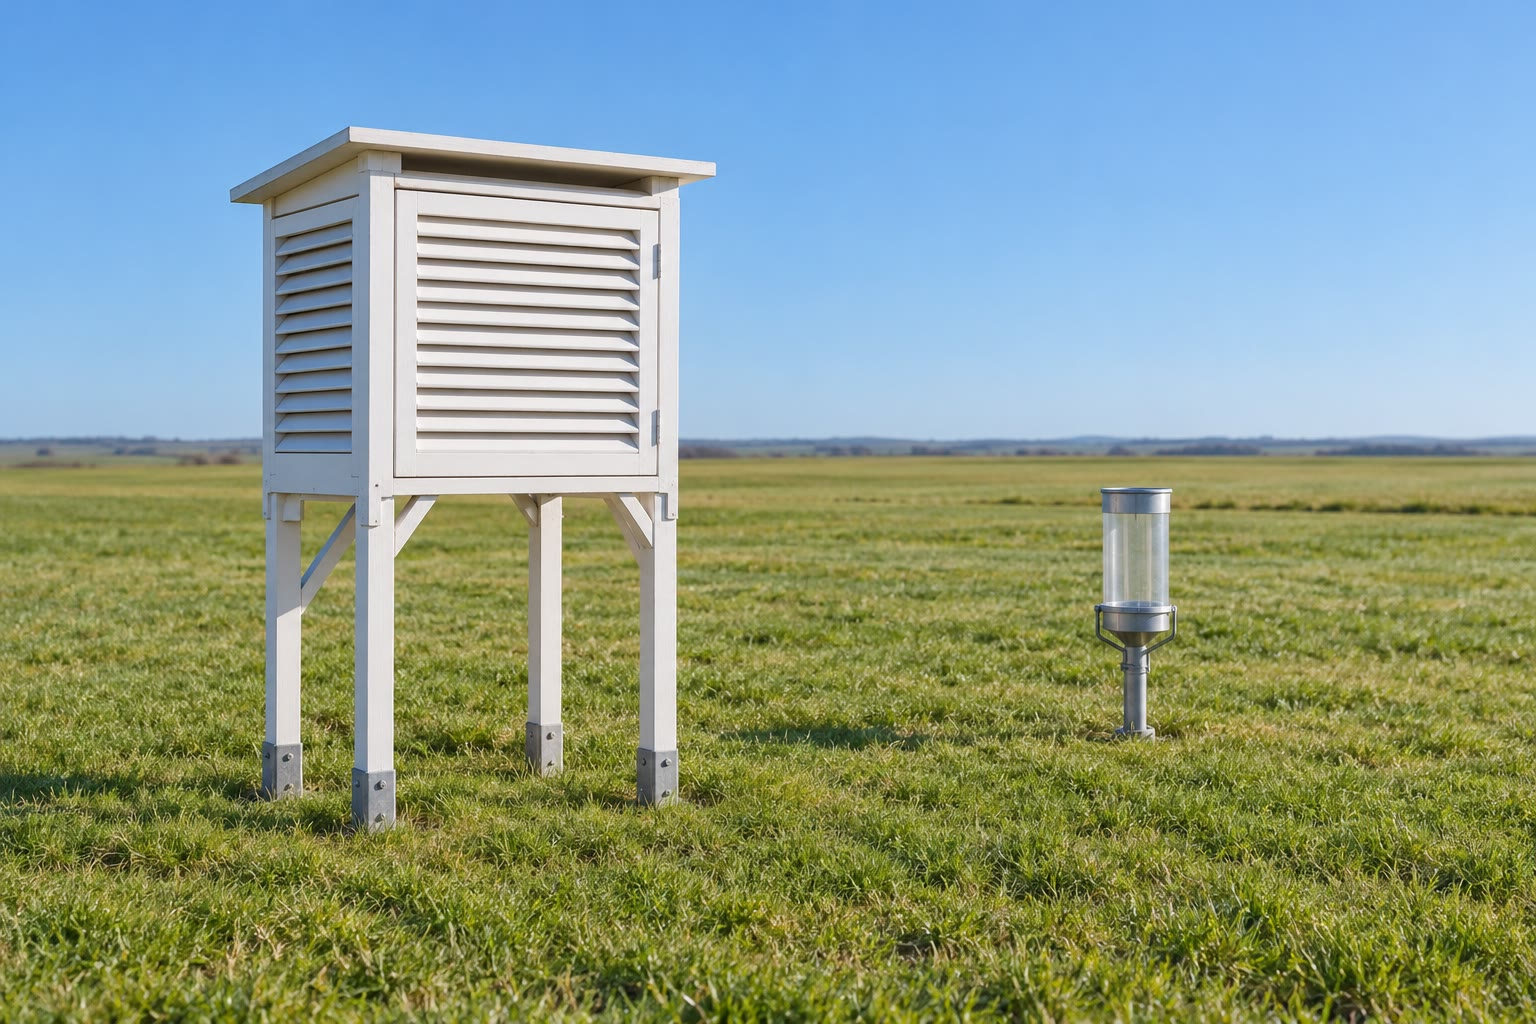
\includegraphics[width=\linewidth]{images/book1/ai/g9-weather-screen.jpg}
\end{minipage}\hfill
\begin{minipage}[c]{0.52\linewidth}\raggedright
{\small एक \omterm{def:g4:clouds-rain-snow:weather-station}{मौसम केंद्र}: पैरों पर खड़ा, झिरीदार दीवारों वाला सफ़ेद बक्सा थर्मामीटरों को
छाया में रखता है जबकि हवा उसमें से होकर बहती है; दाईं ओर एक \omterm{def:g4:clouds-rain-snow:rain-gauge}{वर्षामापी} (एक सामान्य दृश्य
का AI चित्रण)।}
\end{minipage}
\label{fig:g9:climate-past-and-present:screen}
\end{omfigure}

उदाहरण के लिए, वैश्विक तापमान का NASA अभिलेख हर वर्ष की विसंगति 1951--1980 के औसत की
तुलना में देता है, ज़मीनी केंद्रों से और \omterm{def:g2:water-on-earth:ocean}{समुद्र} की सतह के मापों से। दशक-दर-दशक औसत
लेने पर यह एक साफ़ बढ़त दिखाता
है।
% ledger: giss:method, data:gistemp

\begin{omfigure}
\begin{tikzpicture}
\begin{axis}[omrecord, ybar, width=13cm, height=5.6cm, bar width=9pt,
  ymin=-0.45, ymax=1.2, ytick={-0.4,0,0.4,0.8,1.2},
  xtick=data, xticklabels={1880 का दशक, 1890 का दशक, 1900 का दशक, 1910 का दशक, 1920 का दशक, 1930 का दशक, 1940 का दशक, 1950 का दशक, 1960 का दशक, 1970 का दशक, 1980 का दशक, 1990 का दशक, 2000 का दशक, 2010 का दशक, 2020--2025},
  x tick label style={rotate=60, anchor=east, font=\scriptsize},
  ylabel={तापमान विसंगति ($^\circ$C)}, xmajorgrids=false]
  \addplot[fill=omWarm!70, draw=black!50] table[x expr=\coordindex, y=mean_C]
    {figdata/out/grade-9-climate_records-decades.dat};
\end{axis}
\end{tikzpicture}

{\small 1880 के दशक से दशक-दर-दशक वैश्विक सतह तापमान, 1951--1980 के औसत की तुलना
में विसंगति के रूप में; आख़िरी पट्टी छह वर्ष, 2020--2025, लेती है। आँकड़े: NASA
GISTEMP संस्करण~4।}
% ledger: data:gistemp (figdata/grade-9/climate_records.py)
\label{fig:g9:climate-past-and-present:decades}
\end{omfigure}

\begin{definition}[वैश्विक तापन]\label{def:g9:climate-past-and-present:global-warming}
\emph{वैश्विक तापन}\index{वैश्विक तापन} उन्नीसवीं सदी के उत्तरार्ध से, समग्र रूप में,
पृथ्वी की सतह के औसत तापमान की बढ़त
है।
\end{definition}

वर्ष-दर-वर्ष अभिलेख ऊपर-नीचे होता है: एक वर्ष पिछले वर्ष से ठंडा हो सकता है, क्योंकि
\omterm{def:g2:water-on-earth:ocean}{महासागरों} और \omterm{def:g3:continents-and-oceans:continent}{महाद्वीपों} पर पूरे वर्ष का \omterm{def:g1:watching-the-weather:weather}{मौसम} भी बदलता है। इसलिए किसी तापन को मापने के
लिए वैज्ञानिक कई वर्षों के औसतों की तुलना करते हैं, कभी दो अकेले वर्षों की
नहीं।

\begin{omfigure}
\begin{tikzpicture}
\begin{axis}[omrecord, width=13cm, height=5.4cm, xmin=1875, xmax=2030, ymin=-0.6, ymax=1.4,
  xtick={1880,1900,...,2020}, x tick label style={/pgf/number format/1000 sep={}},
  xlabel={वर्ष}, ylabel={तापमान विसंगति ($^\circ$C)},
  legend style={at={(0.2,0.97)}, anchor=north west, draw=none, fill=white, font=\footnotesize}]
  \fill[omWarm!10] (axis cs:1880,-0.6) rectangle (axis cs:1899,1.4);
  \fill[omWarm!10] (axis cs:2015,-0.6) rectangle (axis cs:2024,1.4);
  \addplot[black!70, mark=*, mark size=0.9pt, line width=0.4pt]
    table[x=year, y=anomaly_C] {figdata/out/grade-9-climate_records-annual.dat};
  \addlegendentry{हर वर्ष}
  \addplot[omWarm, line width=2pt] table[x=year, y=mean_C] {figdata/out/grade-9-climate_records-periods.dat};
  \addlegendentry{एक अवधि का औसत}
  \draw[dashed, black!50] (axis cs:1875,0) -- (axis cs:2030,0);
  \node[font=\scriptsize, fill=white, inner sep=1pt] at (axis cs:1889.5,0.45) {1880--1899};
  \node[font=\scriptsize, fill=white, inner sep=1pt] at (axis cs:2019.5,0.3) {2015--2024};
\end{axis}
\end{tikzpicture}

{\small 1880 से 2025 तक हर वर्ष की वैश्विक \omterm{def:g9:climate-past-and-present:anomaly}{तापमान विसंगति} (1951--1980 के औसत की
तुलना में, टूटी रेखा), इस अध्याय की समस्या की दो अवधियों, 1880--1899 और 2015--2024,
के औसतों के साथ। आँकड़े: NASA GISTEMP
संस्करण~4।}
% ledger: data:gistemp (figdata/grade-9/climate_records.py)
\label{fig:g9:climate-past-and-present:annual}
\end{omfigure}

\begin{method}[दो अवधियों के बीच तापन मापना]
\begin{enumerate}
  \item कम से कम दस-दस वर्षों की दो अवधियाँ चुनो, एक शुरुआती और एक बाद की, ताकि अकेले
        वर्षों के उतार-चढ़ाव कट जाएँ।
  \item हर अवधि की वार्षिक विसंगतियों का औसत लो।
  \item बाद वाले औसत में से शुरुआती औसत घटाओ: नतीजा डिग्री में दोनों अवधियों के बीच का
        तापन है।
  \item बताओ कि तुमने कौन-सा अभिलेख और कौन-सी अवधियाँ इस्तेमाल कीं: कोई दूसरा अभिलेख,
        या दूसरी अवधियाँ, थोड़ी अलग संख्या देते हैं।
\end{enumerate}
\end{method}

\begin{example}[1970 के दशक से तापन]
NASA के अभिलेख में दस वर्षों 1970--1979 की विसंगतियों का औसत \qty{0.03}{\degreeCelsius}
है, और 2010--2019 की विसंगतियों का औसत \qty{0.80}{\degreeCelsius}। इन दो दशकों के बीच
का तापन $0.80 - 0.03 = \qty{0.77}{\degreeCelsius}$ है, चालीस वर्षों में: लगभग
\qty{0.19}{\degreeCelsius} प्रति दशक। अकेले वर्ष, जो चालीस वर्ष ही दूर हों, बहुत अलग
जवाब देते: 1976 ($-0.10$) बनाम 2016 (1.01) \qty{1.11}{\degreeCelsius} देता है, पर
1979 (0.16) बनाम 2011 (0.61) केवल
\qty{0.45}{\degreeCelsius}।
\end{example}
% ledger: data:gistemp (figdata/grade-9/climate_records.py: decade_1970s 0.03, decade_2010s 0.80; annual 1976 -0.10, 2016 1.01, 1979 0.16, 2011 0.61)

हवा की कार्बन डाइऑक्साइड मार्च 1958 से सीधे मापी जा रही है, हवाई में मौना लोआ \omterm{def:g4:volcanoes-earthquakes-first-look:volcano}{ज्वालामुखी}
की ढलानों पर लगभग \qty{3400}{m} ऊँचाई पर स्थित एक वेधशाला में। 1959 में उसका वार्षिक
औसत \qty{316}{ppm} था; 2025 तक वह \qty{427}{ppm} पहुँच चुका था, उन \qty{300}{ppm}
से कहीं ऊपर जिनसे वह बर्फ़ के 800\,000 वर्षों में कभी आगे नहीं गया। वह और तेज़ी से बढ़ता
जा रहा है: 1960 के दशक में \qty{1}{ppm} प्रति वर्ष से कम, पिछले दस वर्षों में
\qty{2.5}{ppm} प्रति वर्ष से
ज़्यादा।
% ledger: gml:keeling, data:co2-mlo, data:co2-bereiter (figdata/grade-9/climate_records.py: 315.98, 427.35, 0.86 and 2.63 ppm/yr; ice core max 298.6)

\begin{omfigure}
\begin{tikzpicture}
\begin{axis}[omrecord, width=12cm, height=5cm, xmin=1955, xmax=2030,
  ymin=290, ymax=440, ytick={300,350,400}, xtick={1960,1970,...,2020},
  x tick label style={/pgf/number format/1000 sep={}},
  xlabel={वर्ष}, ylabel={कार्बन डाइऑक्साइड (ppm)}]
  \addplot[black, line width=0.9pt, mark=*, mark size=0.8pt] table[x=year, y=co2_ppm] {figdata/out/grade-9-climate_records-co2.dat};
  \draw[dashed, omWarm] (axis cs:1955,300) -- (axis cs:2030,300);
\end{axis}
\end{tikzpicture}

{\small मौना लोआ, हवाई, पर हवा की कार्बन डाइऑक्साइड, वार्षिक औसत 1959--2025 (NOAA
वैश्विक निगरानी प्रयोगशाला और स्क्रिप्स समुद्र-विज्ञान संस्थान)। \qty{300}{ppm} पर टूटी
रेखा लगभग वह सबसे ऊँचा स्तर है जो अंटार्कटिका की बर्फ़ के 800\,000 वर्षों में
मिला।}
% ledger: data:co2-mlo, data:co2-bereiter (figdata/grade-9/climate_records.py)
\label{fig:g9:climate-past-and-present:co2}
\end{omfigure}

\begin{dated}{2025}
2025 में मौना लोआ पर वार्षिक औसत कार्बन डाइऑक्साइड \qty{427.35}{ppm} थी। NASA
के अभिलेख में 1880 से सबसे गरम वर्ष 2024 था, 1951--1980 की तुलना में
\qty{1.28}{\degreeCelsius} की विसंगति के साथ।
% ledger: data:co2-mlo, data:gistemp (figdata/grade-9/climate_records.py)
\end{dated}

\omterm{def:g2:water-on-earth:ocean}{समुद्र} भी ऊपर उठ रहा है। 1993 से उपग्रहों ने पूरे \omterm{def:g3:continents-and-oceans:globe}{ग्लोब} पर \omterm{def:g2:water-on-earth:ocean}{समुद्र} की सतह की ऊँचाई मापी
है: उनके अभिलेख की प्रवृत्ति रेखा लगभग \qty{3.2}{mm} प्रति वर्ष, यानी तीस वर्षों में लगभग
\qty{10}{cm}, ऊपर उठती है। दो चीज़ें \omterm{def:g2:water-on-earth:ocean}{समुद्र} को ऊपर उठाती हैं: गरम होता पानी फैलता है,
और ज़मीन पर पिघलती बर्फ़ \omterm{def:g2:water-on-earth:ocean}{महासागर} में पानी जोड़ती है। और बर्फ़ सिकुड़ रही है: लगभग हर जगह
\omterm{def:g1:landscapes-around-us:landform}{पहाड़ी} \omterm{def:g8:ice-on-earth:glacier}{हिमनद} पीछे हट रहे हैं, और आर्कटिक की गर्मियों की \omterm{def:g8:ice-on-earth:sea-ice}{समुद्री बर्फ़} ने 1979 से अपने
विस्तार का लगभग आधा खो दिया है (\cref{ch:g8:ice-on-earth})।
% ledger: data:gmsl-lsa (figdata/grade-9/climate_records.py: 3.18 mm/yr; 101 mm 1993-2024), ipcc:b1-ice, nsidc:ice-shelves, data:b1-nsidc-sea-ice

\begin{omfigure}
\begin{tikzpicture}
\begin{axis}[omrecord, width=12cm, height=4.8cm, xmin=1992, xmax=2026,
  ymin=-30, ymax=100, xtick={1995,2000,...,2025},
  x tick label style={/pgf/number format/1000 sep={}},
  xlabel={वर्ष}, ylabel={समुद्र तल (mm)},
  legend style={at={(0.02,0.97)}, anchor=north west, draw=none, fill=white, font=\footnotesize}]
  \addplot[omCold, mark=*, mark size=1.1pt, line width=0.6pt] table[x=year, y=gmsl_mm] {figdata/out/grade-9-climate_records-sea.dat};
  \addlegendentry{वार्षिक औसत}
  \addplot[omWarm, dashed, line width=0.9pt] table[x=year, y=gmsl_mm] {figdata/out/grade-9-climate_records-sea-trend.dat};
  \addlegendentry{प्रवृत्ति रेखा}
\end{axis}
\end{tikzpicture}

{\small उपग्रहों से मापा गया वैश्विक औसत \omterm{def:g4:world-physical-map:altitude}{समुद्र तल}, वार्षिक औसत 1993--2024, एक संदर्भ
स्तर की तुलना में, और उसकी प्रवृत्ति रेखा (NOAA उपग्रह तुंगतामिति
प्रयोगशाला)।}
% ledger: data:gmsl-lsa (figdata/grade-9/climate_records.py)
\label{fig:g9:climate-past-and-present:sea}
\end{omfigure}

\section{जलवायु परिवर्तन और उसके कारण}

\begin{definition}[जलवायु परिवर्तन]\label{def:g9:climate-past-and-present:climate-change}
\emph{जलवायु परिवर्तन}\index{जलवायु परिवर्तन} पृथ्वी की, या किसी क्षेत्र की, \omterm{def:g5:weather-and-climate:climate}{जलवायु} में
ऐसा बदलाव है जो दशकों या उससे ज़्यादा समय तक बना रहे: उसके औसत तापमान, वर्षा, पवनों या
बर्फ़ का बदलाव, न कि केवल एक असामान्य
ऋतु।
\end{definition}

\omterm{def:g5:weather-and-climate:climate}{जलवायु} हमेशा बदलती रही है, जैसा बर्फ़ के कोर दिखाते हैं। नई बात आज के बदलाव की रफ़्तार
है, और उसका कारण। दुनिया भर के वैज्ञानिक \omterm{def:g5:weather-and-climate:climate}{जलवायु} पर जो कुछ प्रकाशित हुआ है उसका नियमित
रूप से आकलन करते हैं, \omterm{def:g9:climate-past-and-present:climate-change}{जलवायु परिवर्तन} पर अंतर-सरकारी पैनल (IPCC) की रिपोर्टों में।
रिपोर्टें तौलती हैं कि हर कथन कितना पक्का है, ध्यान से चुने गए शब्दों के
साथ।

इन रिपोर्टों में नीचे के हर शब्द का एक तय अर्थ है: 100 में वे संभावनाएँ कि कथन सच
है।

\begin{center}
{\small
\begin{tabular}{|l|c||l|c|}
\hline
\emph{लगभग निश्चित} & 99 से 100 & \emph{संभावित} & 66 से 100 \\
\emph{अत्यंत संभावित} & 95 से 100 & \emph{जितना संभावित उतना ही असंभावित} & 33 से 66 \\
\emph{बहुत संभावित} & 90 से 100 & \emph{असंभावित} & 0 से 33 \\
\hline
\end{tabular}}
\end{center}
% ledger: ipcc:likelihood

\noindent कुछ कथनों में इनमें से कोई शब्द नहीं होता: वे तथ्यों के रूप में दिए जाते हैं,
जैसे ``यह \emph{असंदिग्ध} है''। जब तुम \omterm{def:g5:weather-and-climate:climate}{जलवायु} के बारे में कोई समाचार पढ़ो, तो इन शब्दों
को ढूँढो, और ध्यान दो कि समाचार कौन-से शब्द रखता है और कौन-से
छोड़ देता है।
% ledger: ipcc:unequivocal

2021 में प्रकाशित आकलन यह कहता है।
\begin{itemize}
  \item यह \emph{असंदिग्ध} है कि मानव प्रभाव ने वायुमंडल, \omterm{def:g2:water-on-earth:ocean}{महासागर} और ज़मीन को गरम
        किया है।
  \item 2011--2020 का वैश्विक सतह तापमान 1850--1900 की तुलना में लगभग
        \qty{1.1}{\degreeCelsius} ज़्यादा था, और पिछले चार दशकों में से हर एक 1850 के
        बाद के अपने से पहले के किसी भी दशक से ज़्यादा गरम
        था।
  \item 1850--1900 से 2010--2019 तक \emph{संभावित} मानव-जनित तापन 0.8 से
        \qty{1.3}{\degreeCelsius} है, \qty{1.07}{\degreeCelsius} के सबसे अच्छे अनुमान
        के साथ: लगभग पूरा देखा गया तापन। प्राकृतिक कारणों ने मिलकर तापमान को केवल
        $-0.1$ से $+\qty{0.1}{\degreeCelsius}$ तक
        बदला।
  \item 2019 में हवा की कार्बन डाइऑक्साइड कम से कम बीस लाख वर्षों में किसी भी समय से
        ज़्यादा थी (\emph{उच्च विश्वास}); 1750 से वह 47~\% बढ़ चुकी
        थी।
  \item 1990 के दशक से \omterm{def:g8:ice-on-earth:glacier}{हिमनदों} के पीछे हटने का और आर्कटिक की \omterm{def:g8:ice-on-earth:sea-ice}{समुद्री बर्फ़} के सिकुड़ने
        का मुख्य कारण मानव प्रभाव \emph{बहुत संभावित} है; और कम से कम 1971 से \omterm{def:g2:water-on-earth:ocean}{समुद्र}
        के ऊपर उठने का मुख्य कारण भी \emph{बहुत संभावित}
        वही है।
\end{itemize}
% ledger: ipcc:unequivocal, ipcc:gsat-2011-2020, ipcc:decades, ipcc:attribution, ipcc:co2-2myr, ipcc:b1-ice, ipcc:sea-level-obs

\begin{history}[चार्ल्स डेविड कीलिंग का वक्र]
मार्च 1958 में स्क्रिप्स समुद्र-विज्ञान संस्थान के एक युवा रसायनज्ञ, चार्ल्स डेविड
कीलिंग, ने मौना लोआ पर, \omterm{def:g2:water-on-earth:ocean}{समुद्र} से बहुत ऊपर और किसी भी शहर से दूर, हवा की कार्बन
डाइऑक्साइड मापना शुरू किया। उनके माप तब से चल रहे हैं: वे हवा में सीधे मापी गई कार्बन
डाइऑक्साइड का सबसे लंबा अभिलेख हैं, और वर्ष-दर-वर्ष ऊपर उठता जो वक्र वे बनाते हैं, वह
उनका नाम लिए हुए है, \emph{कीलिंग
वक्र}।
% ledger: gml:keeling
\end{history}

तापन कार्बन डाइऑक्साइड के पीछे-पीछे क्यों चलता है? कोयला, तेल और गैस जलाने से कार्बन
डाइऑक्साइड निकलती है; हवा में ज़्यादा कार्बन डाइऑक्साइड का अर्थ है कि सतह से निकलने वाले
अवरक्त प्रकाश का ज़्यादा हिस्सा सोखा और वापस नीचे भेजा जाता है, और सतह गरम होती है।
जलवाष्प, मीथेन और दूसरी ग्रीनहाउस गैसें इस प्रभाव को बढ़ाती हैं। अतीत और वर्तमान सहमत
हैं: बर्फ़ के कोरों में भी और आज के अभिलेखों में भी, पृथ्वी का तापमान और उसकी कार्बन
डाइऑक्साइड साथ-साथ बढ़ते और घटते
हैं।
% ledger: ipcc:attribution, ipcc:co2-2myr

\section{अभ्यास}

\begin{exercise}[$\star$]\label{exo:g9:climate-past-and-present:1}
% ledger: earth:Tbb, earth:Tsurf
(क) ग्रीनहाउस प्रभाव के बिना पृथ्वी की सतह का औसत तापमान क्या होता? (ख) इसके साथ
क्या है? (ग) ग्रीनहाउस प्रभाव सतह को कितने डिग्री गरम करता है? (घ) दो ग्रीनहाउस गैसों
के नाम
बताओ।
\end{exercise}

\begin{exercise}[$\star$]\label{exo:g9:climate-past-and-present:2}
\omterm{def:g1:watching-the-weather:weather}{मौसम} या \omterm{def:g5:weather-and-climate:climate}{जलवायु}? (क) कल पूरे दिन \omterm{def:g4:clouds-rain-snow:precipitation}{बारिश} हुई। (ख) इस क्षेत्र की गर्मियाँ गरम और सूखी होती
हैं। (ग) दुनिया भर में 2010 का दशक 1980 के दशक से ज़्यादा गरम था। (घ) अगला सप्ताह
ठंडा रहेगा।
\end{exercise}

\begin{exercise}[$\star$]\label{exo:g9:climate-past-and-present:3}
% ledger: commons:gisp2-layers
बर्फ़ के कोर के हिस्से की तस्वीर देखो। (क) हिस्सा कितना लंबा है, और उसमें \omterm{def:g4:clouds-rain-snow:precipitation}{हिम} के कितने
वर्ष हैं? (ख) एक वर्ष की परत की औसत मोटाई सेंटीमीटर में निकालो। (ग) किसी \omterm{def:g8:ice-on-earth:ice-sheet}{हिमचादर} की
सबसे गहरी बर्फ़ सबसे पुरानी क्यों होती
है?
\end{exercise}

\begin{exercise}[$\star$]\label{exo:g9:climate-past-and-present:4}
किसी शहर का 1991--2020 का औसत जुलाई तापमान \qty{21.0}{\degreeCelsius} है। उस जुलाई
की \omterm{def:g9:climate-past-and-present:anomaly}{तापमान विसंगति} बताओ जिसका औसत (क) \qty{22.4}{\degreeCelsius}; (ख)
\qty{20.3}{\degreeCelsius}; (ग) \qty{21.0}{\degreeCelsius} हो। (घ) ऋणात्मक विसंगति
का क्या अर्थ है?
\end{exercise}

\begin{exercise}[$\star\star$]\label{exo:g9:climate-past-and-present:5}
% ledger: data:gistemp (figdata/grade-9/climate_records.py)
दशकों वाले स्तंभ चार्ट का उपयोग करो। (क) कौन-से दशक 1951--1980 के औसत से ठंडे थे?
(ख) 1980 के दशक की और 2010 के दशक की विसंगति पढ़ो। (ग) इन दो दशकों के बीच विसंगति
कितनी बढ़ी? (घ) क्या पूरे अभिलेख में एक दशक से अगले दशक तक बढ़त एक-सी
है?
\end{exercise}

\begin{exercise}[$\star\star$]\label{exo:g9:climate-past-and-present:6}
% ledger: data:co2-mlo (figdata/grade-9/climate_records.py)
मौना लोआ पर वार्षिक औसत कार्बन डाइऑक्साइड 1959 में \qty{315.98}{ppm}, 1969 में
\qty{324.62}{ppm}, 2015 में \qty{401.01}{ppm} और 2025 में \qty{427.35}{ppm} थी।
(क) 1959 से 1969 तक प्रति वर्ष औसत बढ़त कितनी थी? (ख) 2015 से 2025 तक? (ग) दूसरी
अवधि में बढ़त कितने गुना तेज़ थी? (घ) 1959 से 2025 तक कार्बन डाइऑक्साइड कितने प्रतिशत
बढ़ी?
\end{exercise}

\begin{exercise}[$\star\star$]\label{exo:g9:climate-past-and-present:7}
% ledger: data:edc-jouzel, data:co2-bereiter
800\,000 वर्षों वाले अभिलेख का उपयोग करो। (क) 800\,000 वर्षों को वैज्ञानिक संकेतन में
लिखो। (ख) हमारे अपने गरम समय से पहले, पिछली बार आज जितना गरम लगभग कितने समय पहले था?
(ग) उस समय हवा में कार्बन डाइऑक्साइड का स्तर क्या था? (घ) क्या तापमान और कार्बन
डाइऑक्साइड एक ही समय पर बढ़ते और घटते
हैं?
\end{exercise}

\begin{exercise}[$\star\star$]\label{exo:g9:climate-past-and-present:8}
% ledger: data:gmsl-lsa (figdata/grade-9/climate_records.py)
\omterm{def:g2:water-on-earth:ocean}{समुद्र} लगभग \qty{3.2}{mm} प्रति वर्ष ऊपर उठता है। (क) 10 वर्षों में यह सेंटीमीटर में
कितना है? (ख) अगर यही दर बनी रहे, तो 2025 और 2100 के बीच वह कितना ऊपर उठेगा? (ग) \omterm{def:g2:water-on-earth:ocean}{समुद्र}
के ऊपर उठने के दो कारण बताओ। (घ) क्या आर्कटिक की \omterm{def:g8:ice-on-earth:sea-ice}{समुद्री बर्फ़} का पिघलना \omterm{def:g2:water-on-earth:ocean}{समुद्र} को ऊपर
उठाता है? समझाओ।
\end{exercise}

\begin{exercise}[$\star\star$]\label{exo:g9:climate-past-and-present:9}
% ledger: ipcc:likelihood
IPCC के शब्दों में, हर कथन के सच होने की 100 में कम से कम कितनी संभावनाएँ हैं? (क) ``यह
\emph{बहुत संभावित} है\ldots'' (ख) ``यह \emph{संभावित} है\ldots'' (ग) ``यह \emph{लगभग
निश्चित} है\ldots'' (घ) कोई अख़बार एक ऐसे कथन के बारे में, जिसे रिपोर्ट \emph{संभावित}
कहती है, लिखता है ``वैज्ञानिक पक्के हैं कि''। क्या ग़लत
है?
\end{exercise}

\begin{exercise}[$\star\star$]\label{exo:g9:climate-past-and-present:10}
एक दोस्त कहता है: ``जहाँ मैं रहता हूँ, यह जाड़ा दस वर्षों में सबसे ठंडा था, इसलिए पृथ्वी गरम
नहीं हो रही।'' \emph{\omterm{def:g1:watching-the-weather:weather}{मौसम}}, \emph{\omterm{def:g5:weather-and-climate:climate}{जलवायु}} और \emph{वैश्विक} शब्दों का उपयोग करके
समझाओ कि यह तर्क क्यों नहीं टिकता।
\end{exercise}

\begin{exercise}[$\star\star\star$]\label{exo:g9:climate-past-and-present:11}
% ledger: data:co2-bereiter, data:co2-mlo, ipcc:co2-2myr, ipcc:erf-2xco2
पिछले \omterm{def:g8:ice-on-earth:ice-age}{हिमयुग} के सबसे ठंडे समय में, लगभग $2 \times 10^4$ वर्ष पहले, हवा में लगभग
\qty{190}{ppm} कार्बन डाइऑक्साइड थी; औद्योगिक युग से ठीक पहले, लगभग
\qty{280}{ppm}; 2025 में, लगभग \qty{427}{ppm}। (क) \omterm{def:g8:ice-on-earth:ice-age}{हिमयुग} से औद्योगिक युग तक कार्बन
डाइऑक्साइड कितनी बढ़ी, और कितने वर्षों में? (ख) औद्योगिक युग से 2025 तक वह कितनी बढ़ी?
1750 को औद्योगिक युग की शुरुआत मानो। (ग) दोनों बढ़तों की तुलना करो: आकार में, और प्रति
वर्ष औसत दर में, वैज्ञानिक संकेतन का उपयोग करके। (घ) IPCC आज के कार्बन डाइऑक्साइड स्तर
के बारे में अतीत की तुलना में क्या कहता
है?
\end{exercise}

\begin{exercise}[$\star\star\star$]\label{exo:g9:climate-past-and-present:12}
% ledger: ipcc:attribution, ipcc:observed-2010-2019
IPCC का आकलन 1850--1900 से 2010--2019 तक देखा गया तापन लगभग
\qty{1.06}{\degreeCelsius} बताता है, और मानव-जनित तापन \emph{संभावित} रूप से 0.8 से
\qty{1.3}{\degreeCelsius} (सबसे अच्छा अनुमान \qty{1.07}{\degreeCelsius}); प्राकृतिक
कारण मिलकर $-0.1$ से $+\qty{0.1}{\degreeCelsius}$ बताए गए हैं। (क) मानव-जनित तापन के
सबसे अच्छे अनुमान की तुलना देखे गए तापन से करो। (ख) क्या अकेले प्राकृतिक कारण देखे गए
तापन को समझा सकते हैं? समझाओ। (ग) इस वाक्य में \emph{संभावित} का क्या अर्थ
है?
\end{exercise}

\section{समस्या: ग्रह का थर्मामीटर}

\begin{problem}[{सप्ताहांत समस्या --- NASA के तापमान अभिलेख से पृथ्वी का तापन निकाला
जाता है, फिर उसे कार्बन डाइऑक्साइड और समुद्र के साथ रखा
जाता है}]
\label{pb:g9:climate-past-and-present:1}
% ledger: data:gistemp, data:co2-mlo, data:gmsl-lsa, ipcc:gsat-2011-2020 (figdata/grade-9/climate_records.py)
तालिका कुछ वर्ष-समूहों के लिए NASA अभिलेख की वैश्विक \omterm{def:g9:climate-past-and-present:anomaly}{तापमान विसंगति} (1951--1980 के
औसत की तुलना में) देती है, और अध्याय के दूसरे
अभिलेख।

\begin{center}
{\small
\begin{tabular}{|l|c|}
\hline
औसत विसंगति, 1880--1899 & \qty{-0.22}{\degreeCelsius} \\
औसत विसंगति, 1951--1980 & \qty{0.00}{\degreeCelsius} \\
औसत विसंगति, 2015--2024 & \qty{0.98}{\degreeCelsius} \\
मौना लोआ पर कार्बन डाइऑक्साइड, 1959 / 2025 & \qty{316}{ppm} / \qty{427}{ppm} \\
उपग्रहों से \omterm{def:g4:world-physical-map:altitude}{समुद्र तल} की प्रवृत्ति, 1993 से & \qty{3.2}{mm} प्रति वर्ष \\
\hline
\end{tabular}}
\end{center}

\noindent\textbf{भाग I --- दशक।}\par\nopagebreak
\begin{enumerate}[beginpenalty=10000]
  \item 1951--1980 की विसंगति ठीक शून्य क्यों है?
  \item 1880--1899, 1951--1980 से गरम था या ठंडा? कितना?
  \item 2015--2024, 1951--1980 से गरम था या ठंडा? कितना?
  \item 1880--1899 की तुलना में 2015--2024 का तापन निकालो।
\end{enumerate}

\noindent\textbf{भाग II --- कार्बन डाइऑक्साइड।}\par\nopagebreak
\begin{enumerate}[resume, beginpenalty=10000]
  \item 1959 और 2025 के बीच कार्बन डाइऑक्साइड कितने ppm बढ़ी?
  \item उसके 1959 के मान के कितने प्रतिशत?
  \item बर्फ़ के कोरों में कार्बन डाइऑक्साइड 800\,000 वर्षों में कभी लगभग
        \qty{300}{ppm} से ऊपर नहीं गई। 2025 का मान उससे कितना ज़्यादा है?
  \item दो वाक्यों में समझाओ कि हवा में ज़्यादा कार्बन डाइऑक्साइड सतह को कैसे गरम करती
        है।
\end{enumerate}

\noindent\textbf{भाग III --- समुद्र।}\par\nopagebreak
\begin{enumerate}[resume, beginpenalty=10000]
  \item तालिका की दर से 1993 से 2025 तक \omterm{def:g2:water-on-earth:ocean}{समुद्र} सेंटीमीटर में कितना ऊपर उठा है?
  \item इस बढ़त के दो कारण बताओ।
  \item IPCC 1850--1900 की तुलना में 2011--2020 का तापन लगभग
        \qty{1.09}{\degreeCelsius} बताता है। क्या प्रश्न~4 का तुम्हारा जवाब उतने ही
        आकार का है? एक कारण बताओ कि दोनों संख्याएँ थोड़ी अलग क्यों
        हैं।
  \item वह वाक्य लिखो जो कोई विज्ञान पत्रकार छाप सकता है: ``उन्नीसवीं सदी के अंत से
        पृथ्वी की सतह लगभग \ldots{} गरम हुई है।''
\end{enumerate}
\end{problem}
